
% !TEX encoding = UTF-8 Unicode

\documentclass[12pt, lettersize]{book}
\usepackage{pdfpages}
\usepackage{graphicx}
\usepackage{scrlayer}
\title{a.le.a parts}
\author{flute}
\date{fdch}
\setcounter{secnumdepth}{-1}
\DeclareNewLayer[
    foreground,
    %textarea,% use only the textarea
    contents={%
      \parbox[b][\layerheight][c]{\layerwidth}
        {\centering this page is intentionally left blank}%
    }
  ]{blankpage.fg}
\DeclarePageStyleByLayers{blank}{blankpage.fg}
\begin{document}
\maketitle
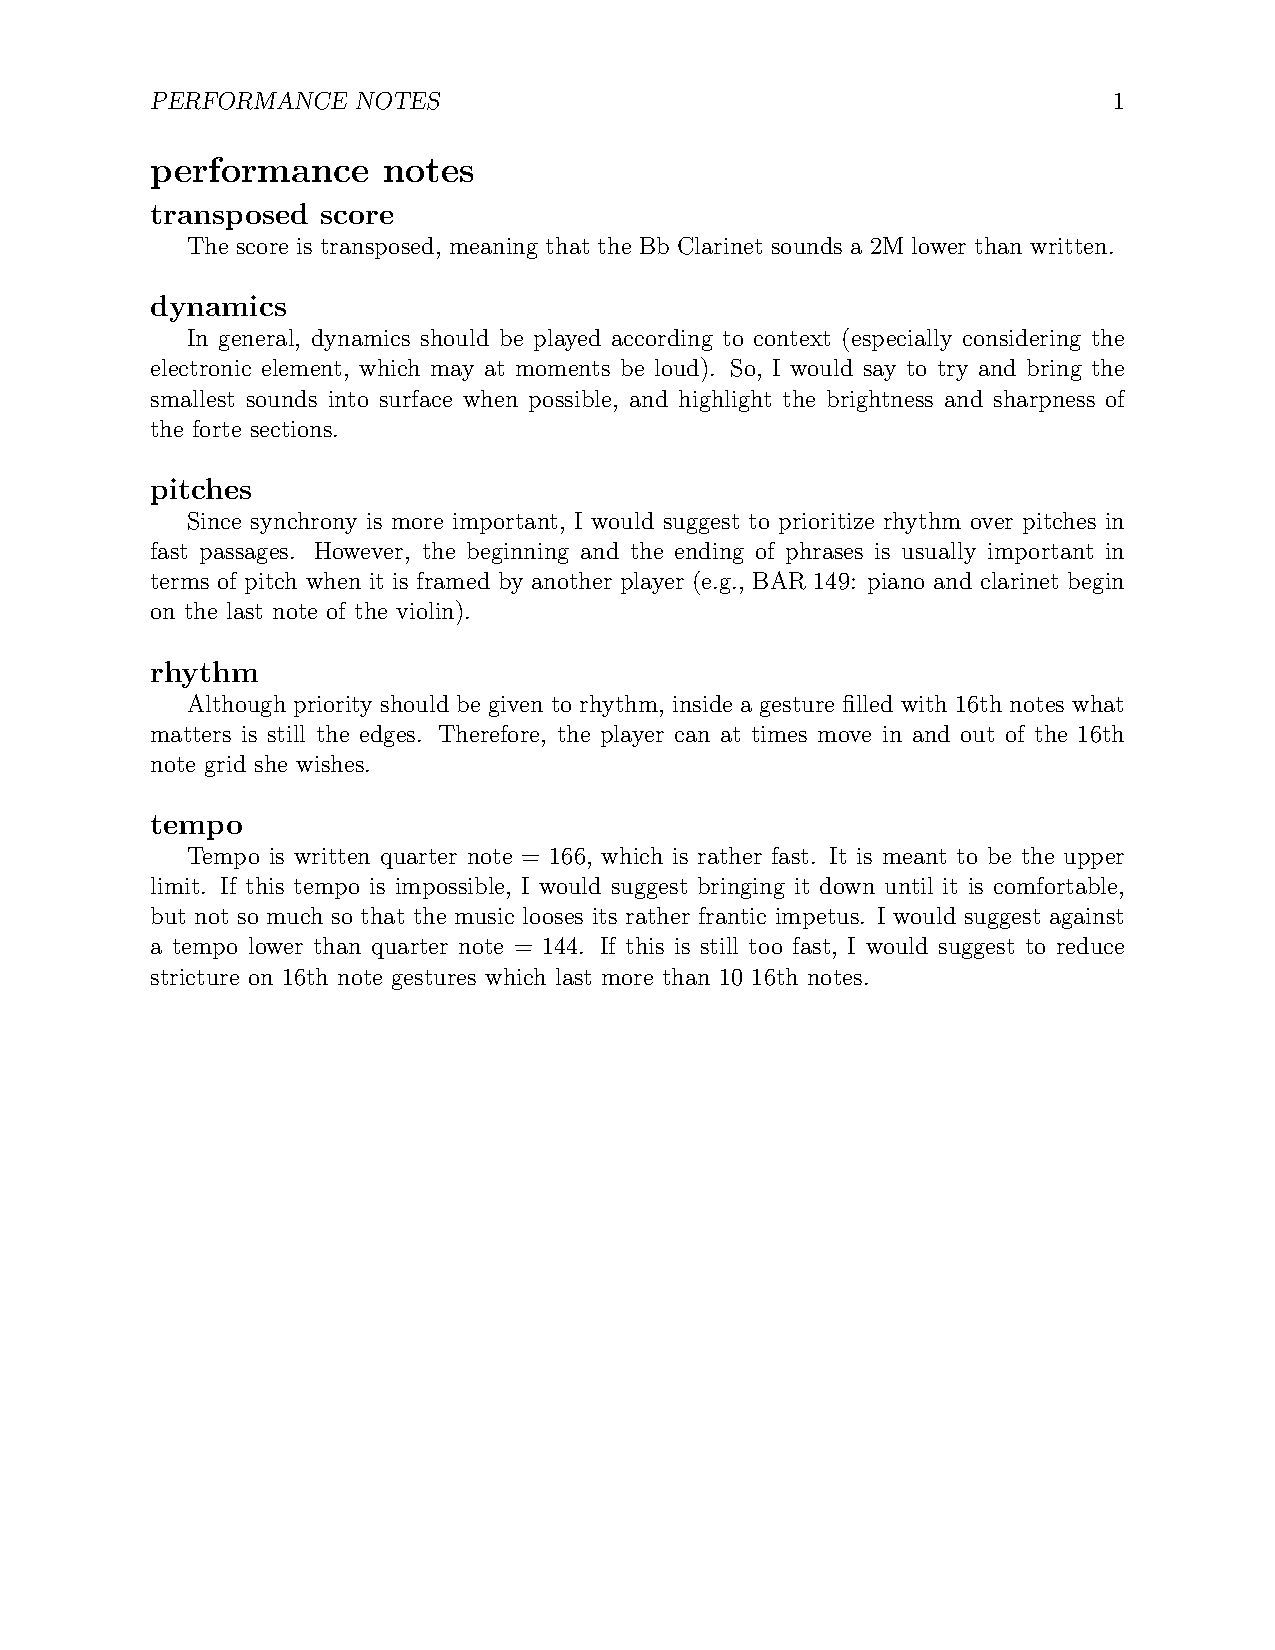
\includepdf[pages =-]{../../alea-head/alea-head.pdf}

\section{notation}\subsection{flute} 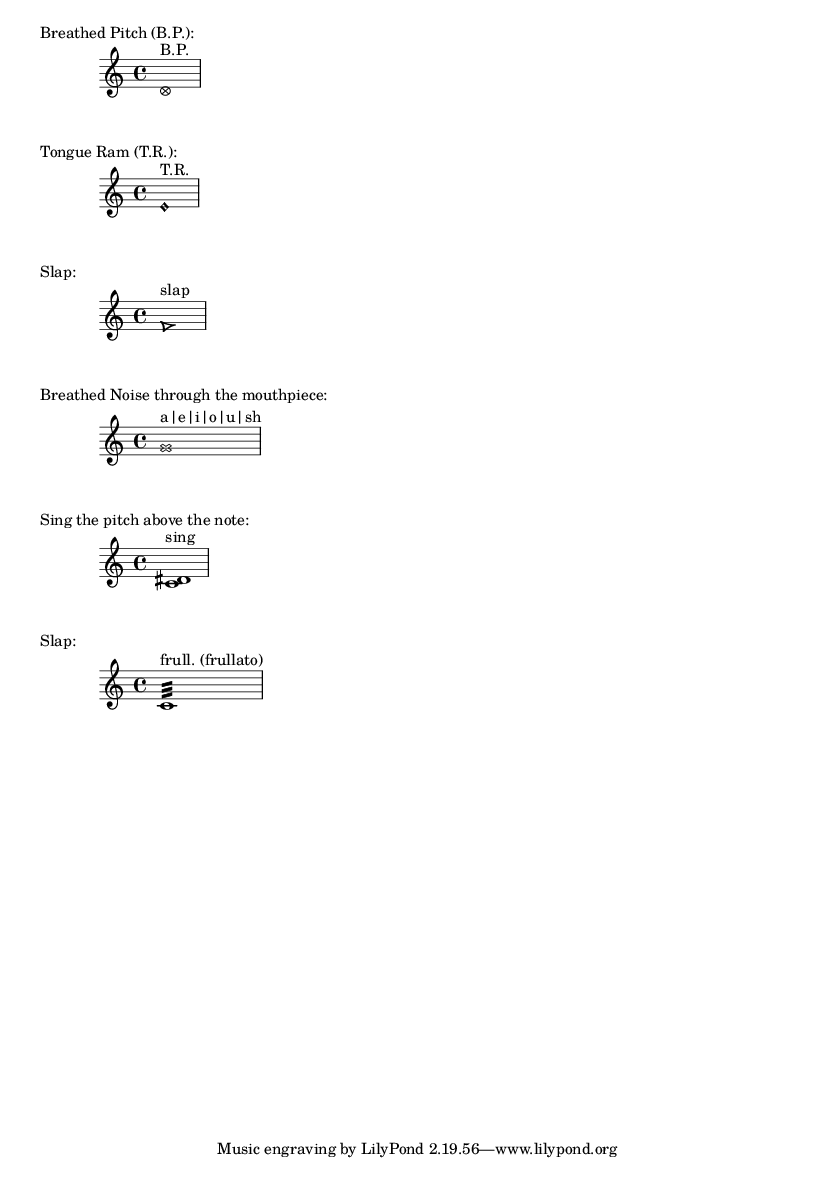
\includegraphics[]{../../../../../reference/flute-notation.png}

\newpage
\null
\thispagestyle{blank}
\newpage

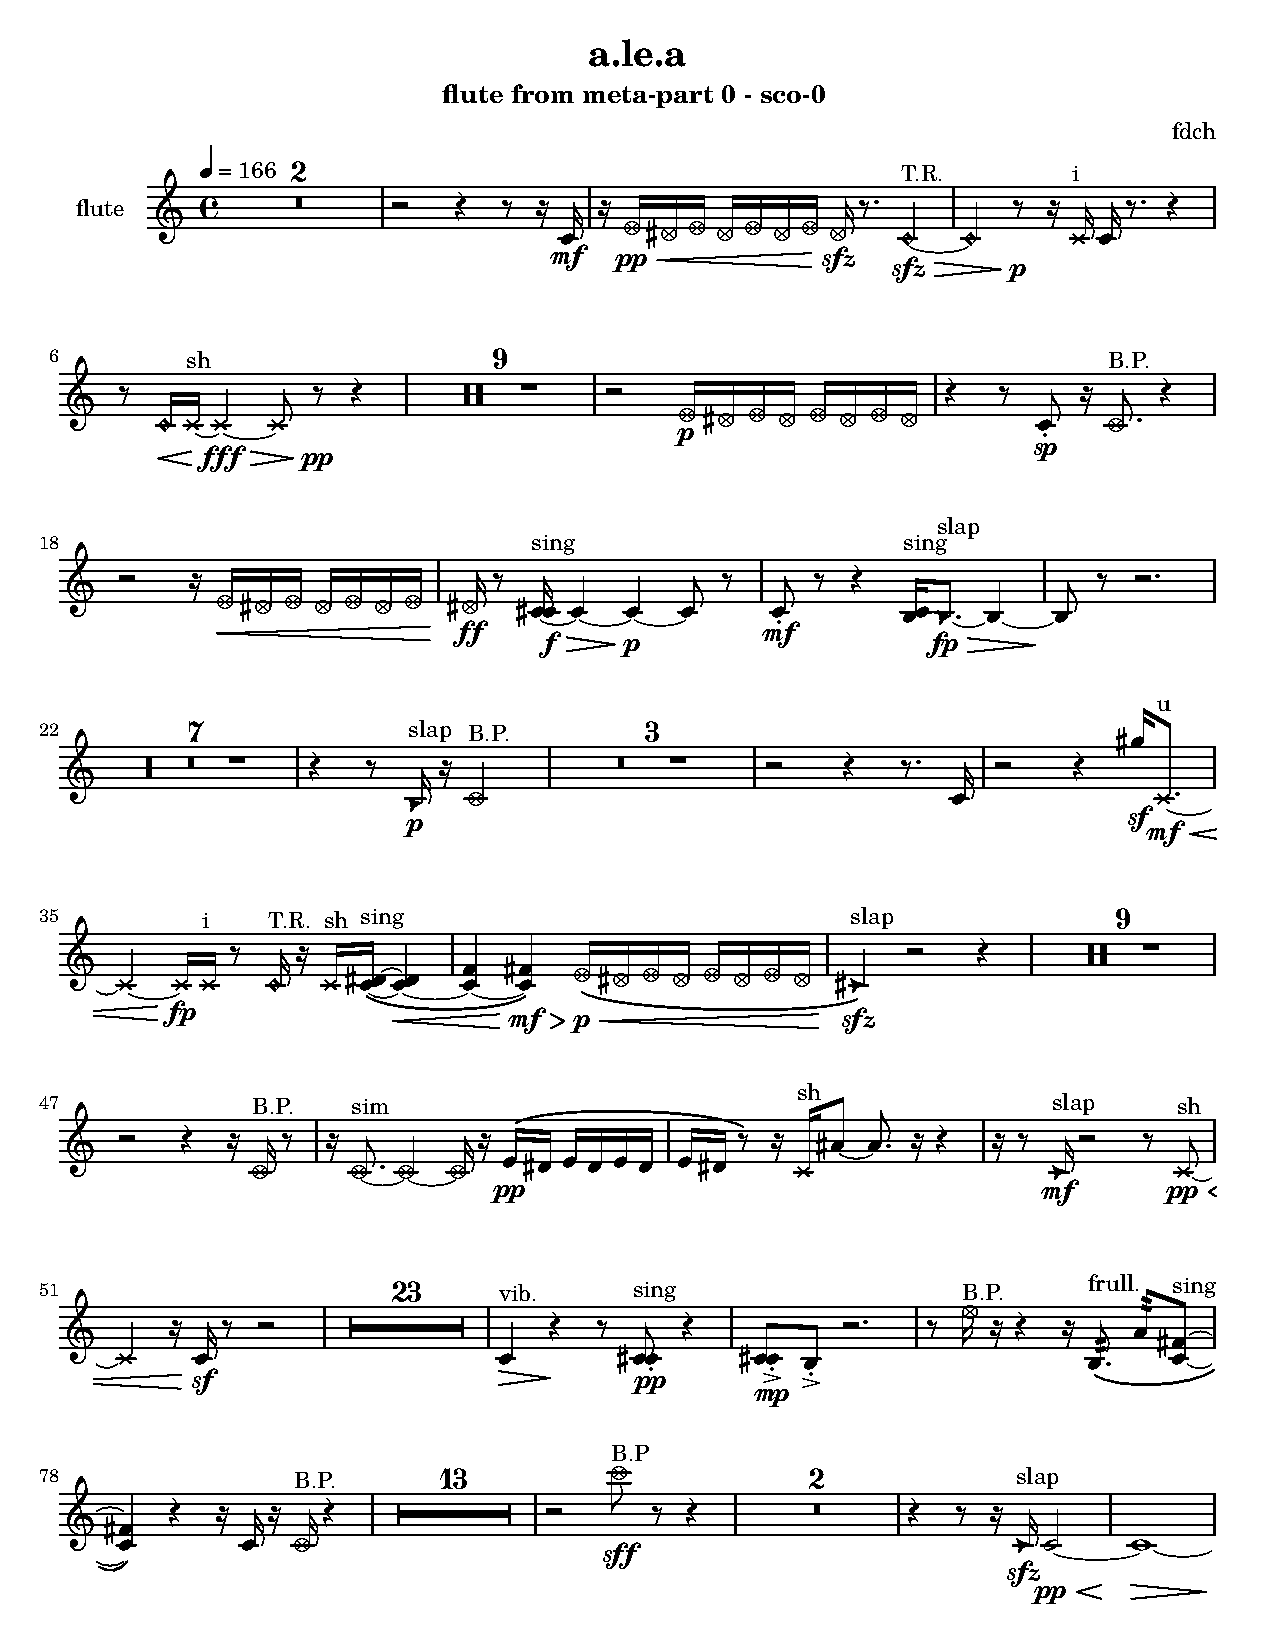
\includepdf[pages =-]{../flute-0.pdf}


\end{document}  

